\documentclass[a4paper,10pt]{article}
\usepackage[utf8]{inputenc}
\usepackage{amssymb}
\usepackage{amsfonts}
\usepackage{amsmath}
\usepackage{enumerate}
\setlength{\parindent}{0pt}
\usepackage[margin=1in]{geometry}

\usepackage{graphicx}
\graphicspath{ {./images/} }

\usepackage{listings}
\usepackage{color}

\definecolor{dkgreen}{rgb}{0,0.6,0}
\definecolor{gray}{rgb}{0.5,0.5,0.5}
\definecolor{mauve}{rgb}{0.58,0,0.82}

\lstset{frame=tb,
  language=C++,
  aboveskip=3mm,
  belowskip=3mm,
  showstringspaces=false,
  columns=flexible,
  basicstyle={\small\ttfamily},
  numbers=none,
  numberstyle=\tiny\color{gray},
  keywordstyle=\color{blue},
  commentstyle=\color{dkgreen},
  stringstyle=\color{mauve},
  breaklines=true,
  breakatwhitespace=true,
  tabsize=3
}
\begin{document}

Jason Qiu

CS 385 Homework Assignment $\#5$

\emph{I pledge my honor that I have abided by the Stevens Honor System.}
\begin{enumerate}
\item \begin{enumerate}[(a)]
	\item \centerline{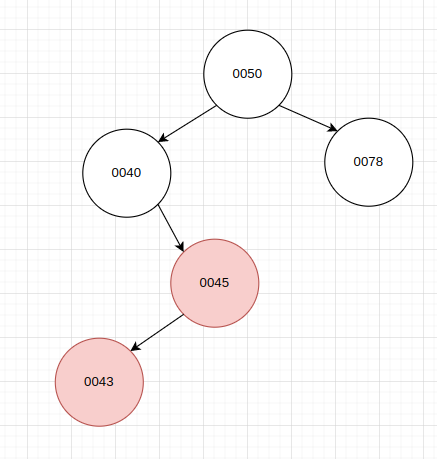
\includegraphics[scale=0.5]{fig1}}
	\item \begin{enumerate}[i.]
		\item Property 4 (no red children for red nodes) is violated.
		\item Case 2b: s's uncle is black and and z is a left child
		\item Set z to z's parent, right-rotate about z
		\item \centerline{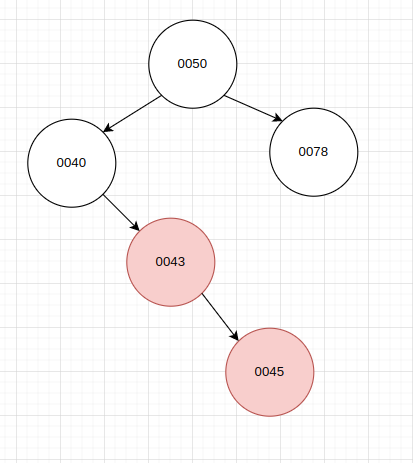
\includegraphics[scale=0.5]{fig2}}
	\end{enumerate}
	\item \begin{enumerate}[i.]
		\item Property 4 (no red children for red nodes) is violated.
		\item Case 3b: z's uncle is is black and z is a right child.
		\item Set z's parent's color to black, set z's grandparent color to red. left-rotate about z's grandparent.
		\item \centerline{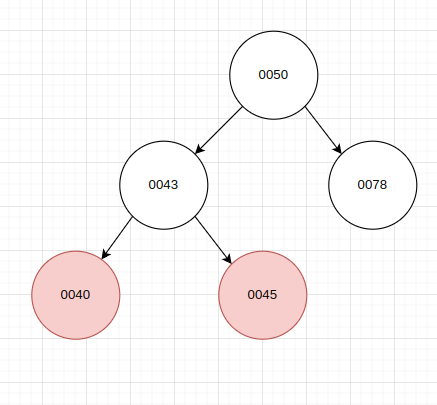
\includegraphics[scale=0.5]{fig3}}
	\end{enumerate}
\end{enumerate}
\item \begin{enumerate}[(a)]
	\item \centerline{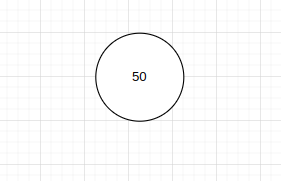
\includegraphics[scale=0.5]{fig4}}
	\item \centerline{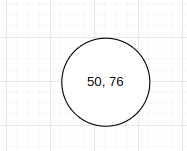
\includegraphics[scale=0.5]{fig5}}
	\item \centerline{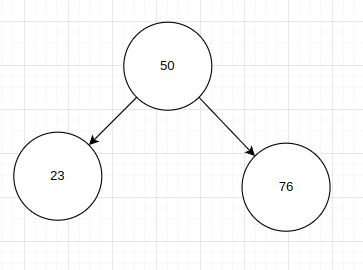
\includegraphics[scale=0.5]{fig6}}
	\item \centerline{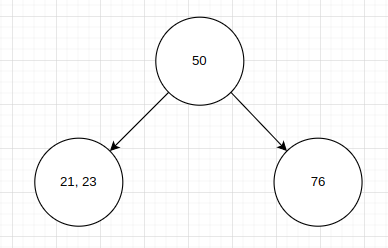
\includegraphics[scale=0.5]{fig7}}
	\item \centerline{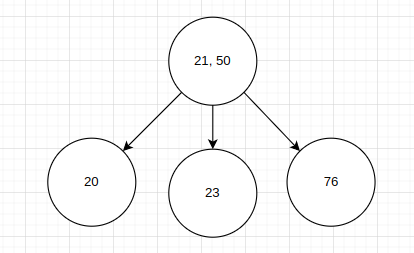
\includegraphics[scale=0.5]{fig8}}
	\item \centerline{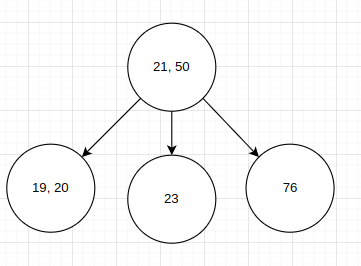
\includegraphics[scale=0.5]{fig9}}
	\item \centerline{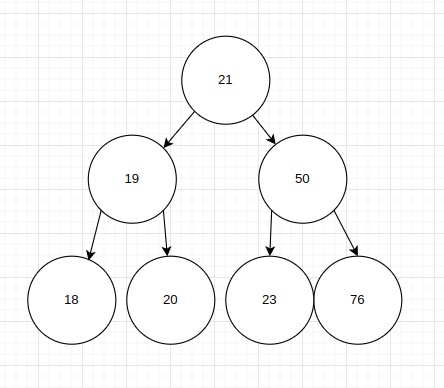
\includegraphics[scale=0.5]{fig10}}
\end{enumerate}

\item \begin{lstlisting}
// Assume A[1..n] denotes an integer array of length n that is indexed starting from 1
ALGORITHM LCM(A[1..n]):
	if n == 1: return A[1]
	if n == 2: return A[1] * A[2] / gcd(A[0], A[1]) // Assume strongly typed language or integer divide default
	return LCM([LCM(the first half of A), LCM(the second half of A)]) // In Python-like list slicing: return LCM([LCM([A[:len(A)//2]), LCM(A[len(A)//2:])])
// Alternate, non-recursive solution
ALGORITHM LCM(A[1..n]):
	result := A[1]
	for i := 2 to n inclusive do:
			result := result * A[i] / gcd(result, A[i]) // Assume strongly typed language or integer divide default
	return result
\end{lstlisting}

\item \begin{enumerate}[(a)]
	\item $p(x) = 7 + x(-4 + x(-2 + x(5 + 4x)))$
	\item \verb|[7, -4, -2, 5, 4]|
	\item 	$p(2) = 95.$

\begin{tabular}{|c|c|c|c|}
		\hline
		$x$ & $p$ & $n$ & $i$ \\
		\hline
		2 & 4 & 4 & 4\\
		\hline
		2 & 13 & 5 & 3\\
		\hline
		2 & 24 & -2 & 2\\
		\hline
		2 & 44 & -4 & 1\\
		\hline
		2 & 95 & 7 & 0\\
		\hline
	\end{tabular}
\item $\frac{4x^4 + 5x^3 - 2x^2 - 4x + 7}{x-2} = 4x^3 + 13x^2 + 24x^1 + 44$ with a remainder of 95:

\begin{tabular}{c|ccccc}
	& 4 & 5 & -2 & -4 & 7\\
	2 & & 8 & 26 & 48 & 88\\
	\hline
	& 4 & 13 & 24 & 44 & $|95$
\end{tabular}
\end{enumerate}

\item \begin{lstlisting}
ALGORITHM LeftRightBinaryExponent(a, b(n)):
	product := 1
	for i := 0 to I inclusive do:
		if b[i] = 1: product := product * a
		a := a * a
	return product
\end{lstlisting}
\end{enumerate}
\end{document}